\clearpage
\section{Structuring scientific work - Workflow management}
\label{sec:workflows}
The process from data generation to a scientific publication can be usually split into individual steps performing only a subset of the complete processing requirend. The separation of these steps can occur on different levels from very coarse like the separation of the experiment and analysis to very fine where each individual processing step is implemented in a independent script.

Workflow management is a concept to organize the individual steps forming a process. The granularity of the steps to manage highly depend on the complexity of the tasks and the diversity of the processing steps. A common and generic example forming a workflow management system is a queueing system used for cluster computing. Here users submit a number of in the simplest case independent jobs (computing steps) which are then depending on the available resources scheduled and distributed to suitable compute resources. This is a simple example, because the individual processing steps typically do not depend on each other and only the required amount of resources and time needs to be taken into account when organizing the execution.

For scientific projects like the Reach-to-Grasp experiment described in \cref{sec:data} there are dependencies between individual steps of the process from data acquisition to publication (see \cref{fig:scidata_metadata_pipeline,fig:scidata_reachgraspio_diagram}). The workflow management concept has been applied in a number of scientifics fields like genomics or imaging data. In these fields a systematic approach to data processing and analysis is required and feasable, since the they are dealing with large and numerous datasets which exceed manual monitoring or processing power \citep[e.g.][]{Palm_2010}.
For these disciplines, there are a number of platforms and tools available to implement pre \& postprocessing as well as analysis processing steps: Galaxy\footnote{Galaxy, \url{https://galaxyproject.org}, RRID:SCR\_006281} an  open, web-based platform providing bioinformatics tools and services for data intensive genomic research, vistrails\footnote{VisTrails, \url{https://www.vistrails.org}, RRID:SCR\_006261} an open-source scientific workflow and provenance management system that provides support for simulations, data exploration and visualization, Taverna\footnote{Taverna, \url{https://taverna.incubator.apache.org}, RRID:SCR\_004437} a scalable, open source \& domain independent tools for designing and executing workflows,  GenePattern\footnote{GenePattern, \url{http://www.broadinstitute.org/cancer/software/genepattern}, RRID:SCR\_003201} a genomic analysis platform that provides access to hundreds of tools for gene expression analysis, proteomics, SNP analysis, flow cytometry, RNA-seq analysis, and common data processing tasks, Renku\footnote{Renku, \url{https://datascience.ch/renku}} an online software platform for reproducible and collaborative data science including workflow management aspects, Terra\footnote{\url{https://terra.bio/}} a scalable platform  for biomedical research for data analysis and collaboration, Ugene \cite{Okonechnikov_2012} a multiplatform open-source software for molecular biology and snakemake\footnote{Snakemake, url{https://snakemake.readthedocs.io/en/stable/}, RRID:SCR\_003475} a Python based language and execution environment for make-like workflows.

In this section we present the usage of snakemake as a workflow management tool as it is domain independent, slim and easily integrates with Python based projects, e.g. to the Reach-to-Grasp and related projects \cref{sec:data}.

\subsection{Workflow management tools - Snakemake}
\label{sec:snakemake}
Snakemake is a generic workflow management tool derived from the build automation tool Make combined with Python features. It is available as bioconda\footnote{\url{https://anaconda.org/bioconda/snakemake}} and PyPi package\footnote{\url{https://pypi.org/project/snakemake}} with the latest version $5.5.4$ being considered here.

We demonstrate the basic features of snakemake based on two minimal workflow examples. The first one (\cref{code:workflows_simple_snakefile}) generates and copies files in two alternative ways and the second, more complex workflow uses two python scripts (\cref{code:workflows_python_scripts}) to generate data using \software{Neo} and visualize it using \software{Matplotlib} (\cref{code:workflows_python_snakefile,fig:python_demo}).

The description of individual steps of a workflow within snakemake is closely related to Make: A processing step is defined via its input and output files (\cref{code:workflows_simple_snakefile} line 11 and 12). The core of a rule is the instruction how to generate the output files based on the input files. Here snakemake offers multiple options based on direct execution of Python scripts or bash scripting. Bash scripts offer the most flexibility and are maked with the \code{shell} keyword (\cref{code:workflows_simple_snakefile} line 13). Within executed shell command references to the input and output files can be used via Python based reformatting of the command before execution. E.g. in \cref{code:workflows_simple_snakefile} line 13 the filename specified by the input of the rule \code{simple\_copy\_rule} (line 11) is automatically copied to the filename specified by the output of the rule by using \code{\{input\}} and \code{\{output\}} in the shell command. The same concept can be used to formulate snakemake rules in a more flexible fashion. E.g. in \cref{code:workflows_simple_snakefile} a set of flexible rules is introduces, which use an additional wildcard \code{\{filename\}} to be able to generate and copy not only files with filename \code{'file.md'}, but any markdown file. Here, the value of the variable \code{\{filename\}} is only determined during the exectution of the workflow. Therefore the same rule can be used multiple times within a workflow with different wildcard parameters. Hereby the value of the wildcard is determined recursively by the required output file.

The dependencies between snakemake rules are evaluated based on required files. By default snakemake uses the first rule within a \code{Snakefile} as main rule and tries to execute this rule. Alternatively snakemake can be called with an filename as an argument. In this case snakemake attempts to build the requested file based on all available rules matching in and output files of rules and checking the availability of basic input files. For this purpose snakemake generates an acyclic directed graph of rule dependencies (e.g. see \cref{fig:workflows_python_snakefile}) and infers all wildcard parameters from this. In case multiple rules can be used for generation of the same file a rule priority order can be be defined (\cref{code:workflows_simple_snakefile} line 1-3). Snakemake only executes rules and creates or overwrites files if the output files of a rule does not exist or the input files have a more recent modification time stamp the output files. This guarantees, that the output files of a snakemake workflow are always based on the most recent version of input files and at the same time minimizes the computational overhead, since only required or outdated files are generated.

Snakemake rule can be executed in dedicated containerized environments. For Python workflows snakemake supports the build of conda environments on a rule level. For each rule the conda environment can be defined via a \code{yaml} files specifying the required dependencies (see \cref{code:workflows_python_snakefile} snakefile line 16 and 23 and environments). Snakemake builds the environment using conda when requiring it the first time and keeps a reference. In case the \code{yaml} environment definition changes, the environment is automatically regenerated.

\cref{code:workflows_python_snakefile} demonstrates a more complex workflow using generic Python scripts for data generating based no the \software{Neo} package and visualization using the Python \software{Matplotlib} package (\cref{code:workflows_python_scripts}. These scripts are implemented to be used as standalone scripts, executed and provided with arguments from the command line. Additionally, they are not relying on a fixed data format, but support any format available in the \software{Neo} framework. This, in combination with the explicit definition of the required python packages in form of \code{yaml} files make the scripts highly flexible and generic, such that they can be easily reused in different contexts and projects. Furthermore, the snakemake implementation of the workflow keeps the genericity of the code by providing flexibility in the used data format, which is defined via an additional configuration \code{yaml} file, and the usage of the usage of wildcards for flexible handling of filenames. The resulting snakemake workflow as well as the output visualization of the randomly generated data can be seen in \cref{fig:python_demo}.


\begin{codeenv}
\textbf{Snakemake header}
\inputminted[firstline=1, lastline=3, linenos,tabsize=2,breaklines, fontsize=\scriptsize]{bash}{figures/workflows/simple_demo.snakefile}
\begin{multicols}{2}
\textbf{Simple rules}
\inputminted[firstline=5, lastline=13, linenos,tabsize=2,breaklines, fontsize=\scriptsize]{bash}{figures/workflows/simple_demo.snakefile}
\columnbreak
\textbf{Flexible rules}
\inputminted[firstline=15, lastline=23, linenos,tabsize=2,breaklines, fontsize=\scriptsize]{bash}{figures/workflows/simple_demo.snakefile}
\end{multicols}
\caption[Minimal snakemake example workflow]{Minimal snakemake example workflow. The workflow consists of two rules, for generation of a markdown file (.md) and conversion to a text file by plain copy of the content into a file with .txt extension. There are two versions of each rule demonstrating snakemake features at different complexities: The simple version of the rule handles filenames explicitely, whereas the flexible version of the rule is using wildcards to handle filenames. To resolve ambiguities between the two versions of the rules, we define a rule priority order in the first lines of the snakemake file.}
\label[codelisting]{code:workflows_simple_snakefile}
\end{codeenv}


\begin{codeenv}
\begin{multicols}{2}
\textbf{Snakefile}\\
\inputminted[firstline=1, lastline=40, linenos,tabsize=2,breaklines, fontsize=\scriptsize]{bash}{figures/workflows/python_demo.snakefile}
\columnbreak
\textbf{Environments}\\
\textbf{plotting\_environment.yaml}
\inputminted[linenos,tabsize=2,breaklines, fontsize=\scriptsize]{yaml}{figures/workflows/envs/plotting_environment.yaml}
\textbf{data\_generation\_environment.yaml}
\inputminted[linenos,tabsize=2,breaklines, fontsize=\scriptsize]{yaml}{figures/workflows/envs/data_generation_environment.yaml}
\textbf{config.yaml}
\inputminted[linenos,tabsize=2,breaklines, fontsize=\scriptsize]{yaml}{figures/workflows/config.yaml}
\end{multicols}
\caption[Snakemake example workflow for data generation and plotting]{Snakemake example workflow for data generation and plotting. The workflow consists of three rules, for data generation, data visualization and specification of the all output files of the workflow. The first two rules can be executed in dedicated conda environments, specified via the \code{conda:} directive and shown at the right. The workflow uses a configuration file (Snakefile line 1, \code{config.yaml}), specifying the format for storing \software{Neo} structures. This specification is also used to provide a constraint for wildcards with the name \code{data\_ext}, which resolves ambiguities between the data generation and visualization rule. The rule \code{all}, is by default executed when snakemake is run, it specifies two required output formats of the workflow. For the visualizaion of the workflow diagram when running the \code{all} rule see \cref{fig:python_demo}.}
\label[codelisting]{code:workflows_python_snakefile}
\end{codeenv}

\begin{figure}
%     \begin{multicols}{2}
    \begin{minipage}[t]{0.4\textwidth}
    \textbf{A}\\
    \includesvg[width=\textwidth, pretex=\relscale{0.8}]{figures/workflows/python_demo_escus}
    \end{minipage}
    \begin{minipage}[t]{0.6\textwidth}
%     \columnbreak\\
    \textbf{B}\\
    \includesvg[width=\textwidth]{figures/workflows/data}\\
    \end{minipage}
    %     \end{multicols}
 \caption[Snakemake example workflow for data generation and plotting]{Snakemake example workflow for data generation and plotting. The workflow diagram (left) and result (right). The workflow consists of two rules of which the \code{plot\_data} rule is executed twice with different parameters to generate the final plot in two file formats (\code{ext: svg}, \code{ex:png}, respecively). Different rules are color coded and the rule name is indicated at the top of each node. The frame style (solid/dashed) indicates if this rule needs to be run to generate a final output file. The arrows indicate the dependencies between the rule executions, rules at the top need to be executed first, since they generate output files that are required as input for the subsequent rules executions.}
\label{fig:python_demo}
\end{figure}


\begin{codeenv}
\begin{multicols}{2}
\textbf{Data generation}
\inputminted[linenos,tabsize=2,breaklines, fontsize=\scriptsize]{python}{figures/workflows/generate_data.py}
\columnbreak
\textbf{Data visualization}
\inputminted[linenos,tabsize=2,breaklines, fontsize=\scriptsize]{python}{figures/workflows/plot_data.py}
\end{multicols}
\caption[Standalone Python scripts used in \cref{code:workflows_python_snakefile}]{Standalone Python scripts used in \cref{code:workflows_python_snakefile}. The two scripts for data generation and visualization contain generic functions, relying on command line parameters to provide the arguments for the function calls (line 21-24 and line 18-21, respectively). The \textbf{data generation} is split into two functions, one for generation of the \software{Neo} structure (\code{generate\_neo\_data}) and one for saving the \software{Neo} structure to disc (\code{save\_neo\_block}). The first function generates a \software{Neo} \code{Block} containing a single \code{AnalogSignal} with randomly generated data (line 4-12). The second function recieves an generic \software{Neo} \code{Block} and saves it in the format specified by the provided filename (line 16-19). If the script is executed from the command line the input parameter \code{filename} is extracted from the command line arguments and both functions are executed consecutively, passing the \software{Neo} \code{Block} from one function the next (line 21-24). The \textbf{data visualization} uses the same concept as the data generation. Here the two internal functions are loading a \software{Neo} block from the specified data source filename (\code{load\_neo\_block}, line 4-7) and visualize the first \code{AnalogSignal} of a given plot, saving the result in a requested filename (code{plot\_analogsignal}, line 9-16). Both functions are called if the script is called from the command line and the two parameters specifying the data location as well as the output plot filename are extracted from the command line arguments.
}
\label[codelisting]{code:workflows_python_scripts}
\end{codeenv}

In addition to the features demonstrated in the example scripts, snakemake integrates well distributed storage concepts, such as Google Cloud Storage\footnote{Google Cloud Storage\url{https://cloud.google.com/storage/}}, DropBox\footnote{DropBox\url{https://www.dropbox.com}} or the secure shell protocol (SSH). Remote file sources are declared in the header of the snakemake file and individual files can be referenced from these sources in the same manner as local files. Besides access to remote files, snakemake also integrates with high-performance compute clusters by supporting common queueing systems such as the slurm workload manager\footnote{slurm, \url{https://slurm.schedmd.com}}. Here, a configuration file can be used to specify the custer job parameters on a rule-level, permitting detailed resource management.

\paragraph{Summary}
We presented the application of basice snakemake workflow features based on two example workflows demonstrating the modularization of a workflow into individual rules and their file-based dependency handling. We highlighted the flexibility of this approach by introducing wildcard based filename handling and explained the snakemake dependency graph. We provide examples of generic standalone Python scripts for seamless integration into snakemake rules and demonstrated advanced configuration features of the workflow via additional configuration files and wildcard constraints. We introduce additional features for integration of remote files and cluster usage.
The presented features make snakemake our tool of choice for the implementation of scientific workflows, as it provides a domain-independent and slim option for workflow definition which integrates well with existing scripted data processing steps.


\todo{inspiration from computer sciences \& industrial software development: Continuous integration \& deployment}



\subsection{Practical application}
Snakemake has been applied in a variety of different fields and projects. Many of the provided examples and tutorials are set in the field of genomics\footnote{\url{https://snakemake.readthedocs.io/en/stable/getting_started/examples.html}}\footnote{\url{https://snakemake.readthedocs.io/en/stable/tutorial/basics.html}} here we present a workflow design in the context of the Vision4Action project, a successor project of Reach-to-Grasp.

\subsubsection{The Vision-For-Action project}
The Vision-For-Action project is building on top of the Reach-to-Grasp project by extending the investigation of motor control only to the interaction of motor and visual activity. For this a modified task is used, involving the continuous integration of visual input and motor control. The experimental hardware is a Real-time visuomotor behavior and electrophysiology recording
(RIVER) setup and consists partially of the same components used in the Reach-to-Grasp experiment. For a detailed description of the recording setup see \cite{deHaan_2018,deHaan_2018a}. The Reach-to-Grasp experiment was extended by an eye as well as hand movement control system and a complex task design including the sequential pointing to up to six targets. To the current date, only a single monkey was recorded in the Vision-For-Action setup.

\paragraph{The task}
In the context of the Vision-For-Action experiment the monkey views a horizontal, semi-transparent mirror on which a red dot is projected corresponding to the location of the monkeys hand below the mirror (\cref{fig:river_setup}). The monkey is trained to initialize a task by moving the hand curser into the area of a central, illuminated target. After a waiting period the central target is deactivated and depending on the task type one or multiple of 6 peripheral targets are illuminated. The to recieve a reward, the monkey has to deactivate all illuminated targets by moving the hand curser into the target. Depending on the task also additional targets might be activated when deactivating the previous target. Two classic task types are implemented currently: The the landing task, in which the monkey is presented a sequence of three peripheral targets, which he has to deactivate by staying in the targets for $100ms$ leading to direct movements to the target. The drawing task, in which the monkey is presented multiple targets at once and can chose an order and route to deactivate these. In this task type the monkey only briefly needs to touch the target with the hand curser leading to very curved movement trajectories. 
\todo{is this already published somewhere? am I permitted to write this?}


\paragraph{The setup}
The RIVER setup consists of four components, which integrates three subsetups covering different modalities. The three components are the recording of the neural activity via a \software{Blackrock} system described in the context of the Reach-to-Grasp experiment, the tracking of eye movement via a an EyeLink system and the tracking / control of the arm movement via a Kinarm motorized exoskeleton of the arm (\cref{fig:river_setup}).

As in the Reach-to-Grasp experiment, neural activity is recorded using Utah array technology. However, instead of a single Utah array implanted in motor cortex, in the Vision-for-Action experiment, an additional Utah array split into $4$ smaller arrays is implanted in visual cortical array. Each Utah array part consists of $6\times6$ electrodes, resulting in a total of $96$ active recording electrodes in motor cortical area M1 and premotor cortex and $32$  active electrodes in vision-related cortical areas V1, V2, 7a and DP. The two Utah arrays are recorded using two recording setups in parallel (see \cref{fig:river_setup} purple panels). This includes two separate connectors implanted contralateral to the Utah arrays, ipsilateral to the active hand of the monkey. The two connectors are during a recording session each connected to a separate headstage including a neural signal amplifier, digitizer and converter. The signals are then optically transmitted to a real-time Neural Signal Processor (NSP) which performs online signal processing (filtering, spike extraction and sorting). In the next step, the processed neuronal signals of each NSP are transmitted to a corresponding offline Cerebus computer for writing to disc and monitoring by the experimenter.

The active arm of the monkey is attached to a Kinarm system, which can be used to track and interfer with the monkey's movement (\cref{fig:river_setup} green panels). The kinarm restricts the hand movement to a horizontal plane below the working space of the monkey and can be used to exert forces onto the monkey's arm. Online feedback of the hand location is provided visually in form of a circular red curser in the working space.

The gaze position of the monkey is tracked using an EyeLink system (\cref{fig:river_setup} blue panels). To be able to record the gaze position, the monkeys head is placed in a plastic head mask, restricting large head movements and providing acces to the reward system. The gaze direction is infered from a video signal showing the cornea reflection of an infrared light source. The raw eye direction signal is online processed using the kinarm real-time system to arrive at the final eye position signal. This conversion depends on the exact location of the monkey's eye with respect to the camera and light source and therefore needs to be calibrated frequently to ensure a stable gaze position recording. For a detailed description of the configuration mechanism and procedure, see \citet{deHaan_2018}.

All online tracked signals, neuronal, kinarm as well as gaze are input to at least one of the  two NSPs, resulting in two sets of \software{Blackrock} files as original data files generated by the RIVER setup.

The experiment control is implemented in a Simulink model on the kinarm realtime computer. This model coordinates the experiment using a Stateflow description of the experimental task and generating corresponding event signals encoding the state of the system. The event codes are unique and globally defined in a generic manner by encoding events using a $16$ bit code. Of the $65536$ possible codes, $1246$ codes are mapped to generic experimental events like a trial start or the beginning of a trial metadata sequence. This leaves $64290$ unused codes, providing sufficient flexibility for future extensions of the schema. For robustness, all event codes come in pairs of two, embracing the metadata information in a start and end bracket. The globally defined experimental codes follow a systematic schema grouping events based on their first digit in six categories: 'Experiment Metadata', 'Trial Metadata', 'Screen Related', 'Exoskeleton Related', 'Other', 'Behaviour Related' and 'Error'. For more details on the global encoding of metadata see \citet{deHaan_2018a}.
For a specific task implementation used in the experiment, a mapping of the globally defined codes to the task specific metadata was defined. This approach permits the global use of generic event codes in the recorded data which at the same time is capable of capturing all task specific metadata. The global event codes generated by the Simulink model are together with hand and gaze location information forwarded to the Blackrock system and saved together with the neuronal signals.

\paragraph{Synchronization}
For coherent data recording from three different systems a shared time frame between all of them is essential for the interpretation of the data. The RIVER setup produces two sets of \software{Blackrock} files since all other signals are integrated online during the recording. The two NSPs provide a synchronization feature, permitting the synchronization of the two systems upon start up of the recording system. To ensure continuous synchrony between the two systems the two NSPs recieve common input from the kinarm system, which can be offline used for validating the common recording time frame.

\paragraph{Data and metadata files}
The RIVER setup generates two sets of \software{Blackrock} recording data files: one containing neural signals from motor and the other from visual cortical areas in the \code{ns6} format. In addition both datasets contain partially identical behavioral signals for the hand, arm and gaze position in the \code{ns2} format(\cref{tab:v4a_recording_files}). In addition also the position of the active target is stored with a $1kHz$ sampling rate as well as the synchronization signals which are shared between the two NSP / Cerebus systems.
Same as for the Reach-to-Grasp experiment, the \code{nev} file also contains online extracted spikes, but in addition it also captures a large amount of structured metadata in form of events, which encode experimental metadata in a generic fashion.
These metadata are complemented by a set of metadata descriptors. These are text files in \code{csv} format, structured in an \software{odMLtables} compatible fashion. These files generated by the experimenter in a manual, but strongly programming aided fashion. The content of these files contains a basic structure for metadata branches to be integrated in an hierarchical \software{odML} metadata collection. A complete set of descriptor files comprises $9$ \code{csv} files and covers all metadata not captured in the event recording file. Essential metadata stored in these \code{csv} files is information about the monkey, the hardware components used, the global and specific codes used in the session, the signal flow for digital and analog signals in the recording setups and the general description of the recording session and meta information about all required descriptor files (\cref{tab:v4a_metadata_files}). Additionally configuration and supplemental files that can not be captured in a csv file but are used during the recording are referenced in the session descriptor. Most of the metadata files are constant across sessions, some change with the task type and only a few need to be generated / tracked explicitely for each session. Nevertheless, we decided to copy even seemingly constant metadata files for each session anew, since during the life time of the experiment also some these metadata can change unexpectedly, e.g. when a part of the setup needs to be replaced due to malfunction.




\begin{sidewaysfigure}
 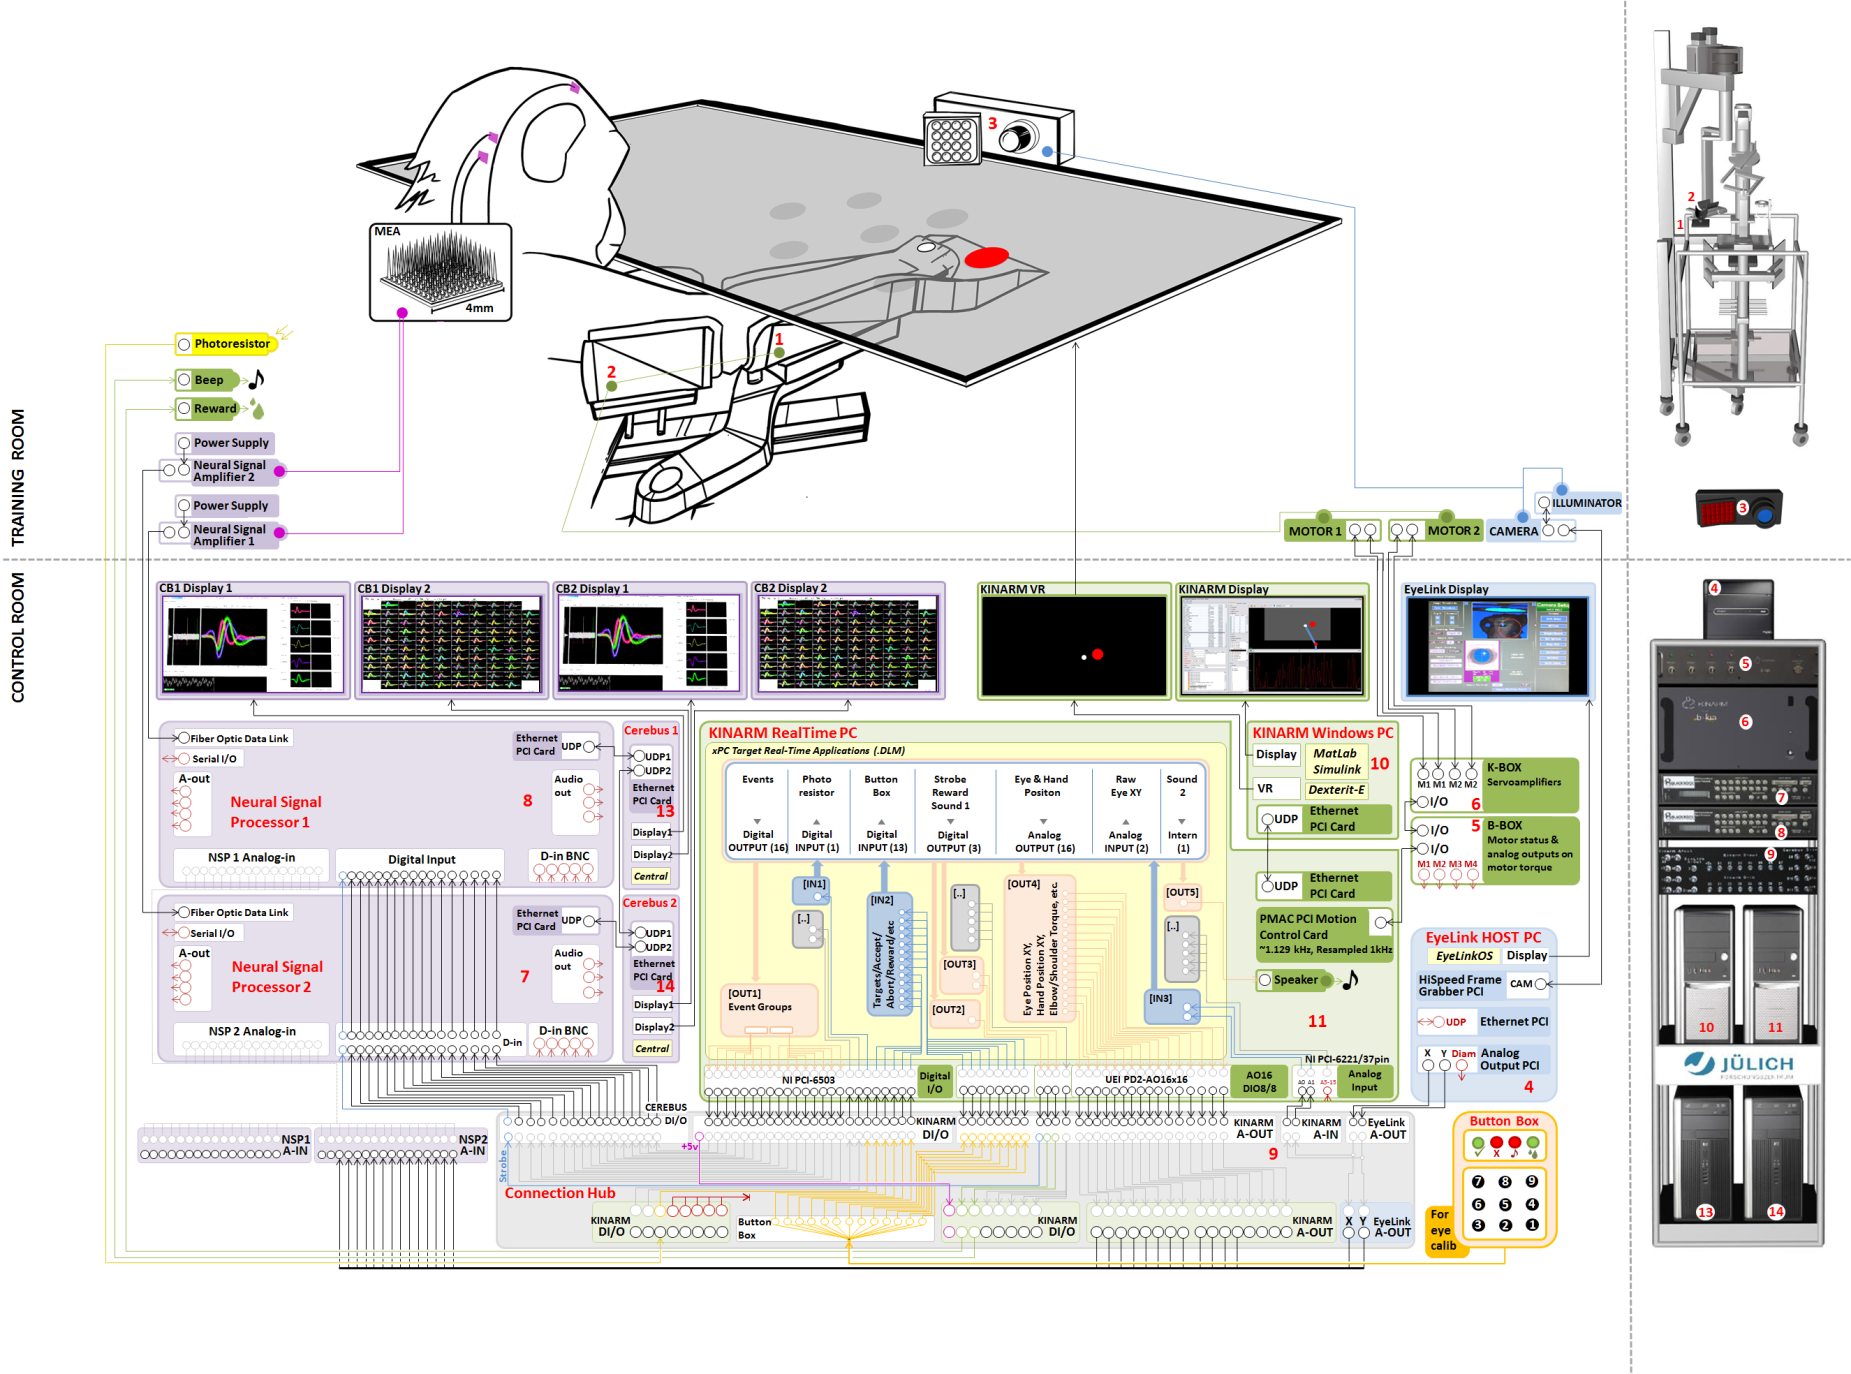
\includegraphics[width=0.8\textwidth]{figures/workflows/river_setup_hardware}
 \caption[The RIVER setup]{The RIVER setup including schematic of hardware components and signal flows. Depicted are the monkey task setup (top right), the recording system and signal flows (bottom left), the monkey chair and kinarm (top right) and the recording hardware rack (bottom right). Figure from \citet{deHaan_2018a}.}
 \label{fig:river_setup}
\end{sidewaysfigure}


\begin{table}[]
\begin{tabular}{|l|l|}
\hline
file format & content                                               \\ \hline
*.ccf       & cerebus configuration                                 \\ \hline
*.nev       & digital events                                        \\
            & \textbullet~ unsorted spiketimes                      \\
            & \textbullet~ spike waveforms                          \\
            & \textbullet~ experiment metadata                      \\
            & \textbullet~ trial metadata                           \\
            & \textbullet~ screen events                            \\
            & \textbullet~ exosceleton events                       \\
            & \textbullet~ behavioural events                       \\
            & \textbullet~ errors                                   \\
            & \textbullet~ ...                                      \\ \hline
*.ns2       & continous signals with $1kHz$ sampling rate           \\
            & \textbullet~ eye (gaze) position                      \\
            & \textbullet~ hand position                            \\
            & \textbullet~ target position                          \\
            & \textbullet~ elbow position                           \\
            & \textbullet~ joint angles / velocities / accelerations \\
            & \textbullet~ synchronization pulses                   \\ \hline
*.n6        & continous signals with $1kHz$ sampling rate           \\
            & \textbullet~ neuronal signals                         \\ \hline
\end{tabular}
\caption[Recording file formats and content in the Vision-for-Action project]{Recording file formats and content in the Vision-for-Action project. The cerebus configuration is saved in a custom \software{Blackrock} configuration format. The nev format contains digital events generated by the NSP based on the neuronal activity (spike detection) and all integrated events from additional hardware systems. Continuous signals are stored in different files depending on the sampling resoulution. At a low sampling resolution of $1kHz$ the ns2 signal contains behavioral signals whereas the neuronal high sampling resolution signals are stored in the ns6 file.}
\label{tab:v4a_recording_files}
\end{table}

\begin{table}[]
\scriptsize
\begin{tabular}{lll}
\textbf{Descriptor}                                & \textbf{Content}                                                                                                       & \textbf{Generation}                                                                  \\ \hline
\multicolumn{1}{|l|}{session}                      & \multicolumn{1}{l|}{\textbullet~ session name}                                                                         & \multicolumn{1}{l|}{once per session}                                                \\
\multicolumn{1}{|l|}{}                             & \multicolumn{1}{l|}{\textbullet~ relevant metadata files}                                                              & \multicolumn{1}{l|}{semi-automatic}                                                  \\
\multicolumn{1}{|l|}{}                             & \multicolumn{1}{l|}{\textbullet~ task type}                                                                            & \multicolumn{1}{l|}{visual cross check}                                              \\
\multicolumn{1}{|l|}{}                             & \multicolumn{1}{l|}{\textbullet~ ...}                                                                                  & \multicolumn{1}{l|}{}                                                                \\ \hline
\multicolumn{1}{|l|}{subject}                      & \multicolumn{1}{l|}{\textbullet~ species}                                                                              & \multicolumn{1}{l|}{onetime, static}                                                 \\
\multicolumn{1}{|l|}{}                             & \multicolumn{1}{l|}{\textbullet~ active hand}                                                                          & \multicolumn{1}{l|}{}                                                                \\
\multicolumn{1}{|l|}{}                             & \multicolumn{1}{l|}{\textbullet~ training}                                                                             & \multicolumn{1}{l|}{}                                                                \\
\multicolumn{1}{|l|}{}                             & \multicolumn{1}{l|}{\textbullet~...}                                                                                   & \multicolumn{1}{l|}{}                                                                \\ \hline
\multicolumn{1}{|l|}{kinarm}                       & \multicolumn{1}{l|}{\textbullet~ hardware specifications}                                                              & \multicolumn{1}{l|}{onetime, static}                                                 \\
\multicolumn{1}{|l|}{}                             & \multicolumn{1}{l|}{\textbullet~ programming software}                                                                 & \multicolumn{1}{l|}{}                                                                \\
\multicolumn{1}{|l|}{}                             & \multicolumn{1}{l|}{\textbullet~ ...}                                                                                  & \multicolumn{1}{l|}{}                                                                \\ \hline
\multicolumn{1}{|l|}{eyelink}                      & \multicolumn{1}{l|}{\textbullet~hardware specifications}                                                               & \multicolumn{1}{l|}{onetime, static}                                                 \\
\multicolumn{1}{|l|}{}                             & \multicolumn{1}{l|}{\textbullet~ software specifcations}                                                               & \multicolumn{1}{l|}{}                                                                \\
\multicolumn{1}{|l|}{}                             & \multicolumn{1}{l|}{\textbullet~ ...}                                                                                  & \multicolumn{1}{l|}{}                                                                \\ \hline
\multicolumn{1}{|l|}{blackrock}                    & \multicolumn{1}{l|}{\textbullet~ Utah arrays}                                                                          & \multicolumn{1}{l|}{onetime, static}                                                 \\
\multicolumn{1}{|l|}{}                             & \multicolumn{1}{l|}{\textbullet~ connectors}                                                                           & \multicolumn{1}{l|}{}                                                                \\
\multicolumn{1}{|l|}{}                             & \multicolumn{1}{l|}{\textbullet~ physical properties}                                                                  & \multicolumn{1}{l|}{}                                                                \\
\multicolumn{1}{|l|}{}                             & \multicolumn{1}{l|}{\textbullet~ ...}                                                                                  & \multicolumn{1}{l|}{}                                                                \\ \hline
\multicolumn{1}{|l|}{analog\_communication}        & \multicolumn{1}{l|}{\textbullet~ hardware specifications}                                                              & \multicolumn{1}{l|}{onetime, static}                                                 \\
\multicolumn{1}{|l|}{}                             & \multicolumn{1}{l|}{\textbullet~ pin mapping}                                                                          & \multicolumn{1}{l|}{}                                                                \\
\multicolumn{1}{|l|}{}                             & \multicolumn{1}{l|}{\textbullet~ ...}                                                                                  & \multicolumn{1}{l|}{}                                                                \\ \hline
\multicolumn{1}{|l|}{digital\_communication}       & \multicolumn{1}{l|}{\textbullet~ hardware specifications}                                                              & \multicolumn{1}{l|}{onetime, static}                                                 \\
\multicolumn{1}{|l|}{}                             & \multicolumn{1}{l|}{\textbullet~ pin mapping}                                                                          & \multicolumn{1}{l|}{}                                                                \\
\multicolumn{1}{|l|}{}                             & \multicolumn{1}{l|}{\textbullet~ ...}                                                                                  & \multicolumn{1}{l|}{}                                                                \\ \hline
\multicolumn{1}{|l|}{codes\_global}                & \multicolumn{1}{l|}{\textbullet~ code mapping \& definition}                                                           & \multicolumn{1}{l|}{onetime, static}                                                 \\ \hline
\multicolumn{1}{|l|}{codes\_task}                  & \multicolumn{1}{l|}{\textbullet~ mapping of global codes to}                                                           & \multicolumn{1}{l|}{once per task type}                                              \\
\multicolumn{1}{|l|}{}                             & \multicolumn{1}{l|}{\hspace{1cm} task specific metadata}                                                               & \multicolumn{1}{l|}{static}                                                          \\ \hline
\textbf{Additional metadata files}                 &                                                                                                                        &                                                                                      \\ \hline
\multicolumn{1}{|l|}{task description (pdf)}       & \multicolumn{1}{l|}{\begin{tabular}[c]{@{}l@{}}extensive human readable task description\\ with sketches\end{tabular}} & \multicolumn{1}{l|}{\begin{tabular}[c]{@{}l@{}}once per task,\\ static\end{tabular}} \\ \hline
\multicolumn{1}{|l|}{task model (mdl)}             & \multicolumn{1}{l|}{model description file as used by SimuLink}                                                        & \multicolumn{1}{l|}{\begin{tabular}[c]{@{}l@{}}once per task,\\ static\end{tabular}} \\ \hline
\multicolumn{1}{|l|}{task parameter file (dtp)}    & \multicolumn{1}{l|}{task parameter file as used by SimuLink}                                                           & \multicolumn{1}{l|}{\begin{tabular}[c]{@{}l@{}}once per task,\\ static\end{tabular}} \\ \hline
\multicolumn{1}{|l|}{target picture (png)}         & \multicolumn{1}{l|}{image used for visual targets}                                                                     & \multicolumn{1}{l|}{onetime}                                                         \\ \hline
\multicolumn{1}{|l|}{calibration parameters (mat)} & \multicolumn{1}{l|}{parameters of the calibration model}                                                               & \multicolumn{1}{l|}{onetime}                                                         \\ \hline
\multicolumn{1}{|l|}{calibration data (mat)}       & \multicolumn{1}{l|}{data used for calibration}                                                                         & \multicolumn{1}{l|}{once per calibration}                                            \\ \hline
\end{tabular}
\caption[Metadata files in the Vision-for-Action project]{Metadata descriptors and supplementary files in the Vision-for-Action project. Nine \code{csv} descriptor files are required for a complete description of the experiment. Most of these only need to be generated once as the contained data should be static. Only the session descriptor needs to be adjusted each session as well as the task code descriptor if a new task was introduced. There are six additional files which provide supplemental metadata information. These provide additional configuration and image material used during the recording.}
\label{tab:v4a_metadata_files}
\end{table}

\subsection{Metadata workflow in the Vision-for-Action project}

Based on the metadata source files described in \cref{tab:v4a_metadata_files} we designed a workflow for metadata collection and enrichment which consisting processing steps that can be classified into one of five processing categories (\cref{fig:v4a_metadata_workflow_rulegraph}). The implementation of the workflow is still work in progress, but the basic concepts and completed implementation steps are presented in the following. We implement the workflow using snakemake in combination with python scripts, which are implemented in a standalone fashion as described in \cref{sec:snakemake} (\cref{code:workflows_python_scripts}). In the context of this workflow we term these standalone python scripts 'application' (\textbf{app}). Each app performs only a single, definite processing step based on as few input files as possible, to avoid unnessesary dependencies.

\paragraph{Grouping of apps}
We grouped similar apps according to their interface. This way a single rule can handle multiple apps in case they are having a similar dependency structure and require the same parameters. An example for this are \code{metadata apps}(\cref{fig:v4a_metadata_workflow_rulegraph}, green panel). This rule covers all apps, which generate metadata based on the original recording data and generate an \software{odMLtables} compatible csv file summarizing the extracted metadata or processing results. In constrast to this \code{data\_apps} extend the original data (in the \software{Neo} representation) and generate an \software{odMLtables} compatible \code{csv} file. Each generated \code{csv} file is saved with an app-specific filename and typically contains only a few values of additional metadata, since apps are modularized to cover very specific tasks.
In the current workflow, metadata and data apps are implemented in a flexible manner, as these apps are located in a dedicated folder. All apps in these folders are automatically included in the workflow and are executed by the the \code{run\_metadata\_app} and \code{run\_data\_app} rules (\cref{code:v4a_workflow_snakemake_rule}.

Two minimal examples depicting two subsets of the workflow are shown in \cref{fig:v4a_metadata_workflow_dag}. Here we focus on the integration of the original \code{csv} descriptors into a single \software{odML} file as well as the execution of preprocessing steps (\cref{fig:v4a_metadata_workflow_dag}A and B, respecively). The general  dependencies between the corresponding rules is visible in \cref{fig:v4a_metadata_workflow_rulegraph}, whereas the executions of the rule with varying parameters is depicted in \cref{fig:v4a_metadata_workflow_dag}. The large number of apps handled by some of the rules prevents a visualization of the complete workflow in this context, hence only a small selection of apps is depicted.
In the first, descriptor conversion example, the metadata descriptors first all \code{csv} descriptors need to be copied to the working directory of the workflow as the descriptors are stored together with the original data in a read-only folder. This prevents unintentional changes of the original data and makes the workflow therefore less error-prone. Each descriptor files in copied by an application of the \code{copy\_descriptors} rule with parameters specifying the descriptor. These copies serve as an input for the \code{csv\_to\_odml} rule, which permits the conversion of any \software{odMLtables} compatible \code{csv} file to the \software{odML}. This step is also run for all descriptors separately. In addition the \code{csv\_to\_odml} rule also requires an \software{odML} style sheet for the user friendly visualization of the \software{odML} file via \code{html}. This is a required input for all realizations of the \code{copy\_to\_csv} rule, but will only be executed once as the \code{add\_odML\_style\_sheet} rule does not depend on the identity of the descriptor, but downloads the style sheet once to the descriptor working directory. Finally, the \code{integrate\_descriptors} rule uses all previously create \software{odML files} as input and integrates all \software{odML} files referenced in the session \software{odML} into a common \software{odML} file.
In the second, data and metadata preprocessing example, two types of preprocessing steps are performed: preprocessing and metadata extractraction with and without extension of the neuronal data set. Apps that only access the original neuronal data to extract metadata (e.g. data integrity checks) are coordinated by the \code{run\_metadata\_app} and access the neuronal data in the original \software{Blackrock} format. Preprocessing steps that extend the original neuronal dataset (e.g. by performing spike sorting) require a data representation in the generic, open source \software{Nix} format (see \cref{sec:nix_format}), to be able to successively extend the dataset. The initial conversion from the \software{Blackrock} to the \software{Nix} format is performed by the \code{data\_to\_nix} rule. Here, the order of execution of the data apps is not specified in the workflow, hence only independent data processing steps can be implemented with this mechanism. Future extensions by interdependent preprocessing steps can be added as complementary rules with a higher rule priority order than the \code{run\_data\_app} rule (see \cref{code:workflows_simple_snakefile} line 1-3).

Currently implemented and envisioned metadata apps cover both aspects of data quality assurance as well as extraction of essential information for easy access. Some examples for data quality assurance are listed below:
\begin{itemize}
 \item check for the existance of all recording files
 \item check for the integrity of events recorded with both NSP systems. This ensures synchronicity of the datasets between the two independent \software{Blackrock} recording systems.
 \item check for integrity of online extracted spikes and continously sampled raw data. In case of a silent data packet loss during the recording, spike and continous data are not aligned from the time point of data loss (see also \cref{sec:additional_features_gaps}). The occurrence of a gap can be automatically detected with a high probablity.
\end{itemize}

Examples for extraction of basic metadata are:
\begin{itemize}
  \setlength{\itemsep}{1pt}
  \setlength{\parskip}{0pt}
  \setlength{\parsep}{0pt}
 \item the collection of channel specific information in a specific branch of the metadata collection
 \item the evaluation whether a session was already offline spike sorted
 \item the evaluation of the monkey's performance
 \item the creation of overview plots of 
 \begin{itemize}
  \item the basic recording data
  \item detected hyper-synchronous events in the spiking data and their complexity distribution (see \cref{sec:spike_data_quality})
 \end{itemize}
\end{itemize}

In constrast to metadata apps, data apps extent the \software{Neo} data structure. Some examples of implemented and envisioned data apps are:
\begin{itemize}
  \setlength{\itemsep}{1pt}
  \setlength{\parskip}{0pt}
  \setlength{\parsep}{0pt}
 \item the detection of cross talk between individual electrodes and annotation of the corresponding recording traces
  \item the detection and annotation of hyper-synchronous events in spiking data (see \cref{sec:spike_data_quality})
 \item the extraction of events from continous recording signals such as
 \begin{itemize}
  \item the extraction of saccades from the eye (gaze) position
  \item the segmentation of the hand movement into subtrajectories
 \end{itemize}
\end{itemize}


\paragraph{Code and data folder structure}
The workflow project is organized in the following structure:\\

\renewcommand*\DTstylecomment{\color{gray}\textit}
\renewcommand*\DTstyle{\textcolor{black!90}}
\begin{minipage}[t]{\textwidth}
\dirtree{%
.1 workflow folder\DTcomment{workflow repository folder}. 
.2 Snakefile\DTcomment{definition of snakemake workflow}.
.2 config.yaml\DTcomment{configuration of snakemake workflow}.
.2 config\_template.yaml\DTcomment{template for setting up config.yaml}.
.2 envs.
.3 metadata\_env.yaml\DTcomment{contains conda Python environment definitions}.
.2 scripts\DTcomment{contains python scripts coordinated by snakemake}.
.3 data\_apps\DTcomment{contains data enriching apps}.
.3 metadat\_apps\DTcomment{contains metadata aggregating apps}.
.3 infrastructure\DTcomment{contains general purpose apps}.
.3 utilities.
.4 util.py\DTcomment{contains utility functions used by apps}.
.3 tests\DTcomment{contains test suite for apps}.
.3 app\_example.py\DTcomment{template implementation of an app}.
}
\ \\
\end{minipage}

The separation of different types of apps into subfolders permits to automatically collect data and metadata applications during the runtime of the snakemake workflow. This avoids hard coding of app names in the workflow and provides a more flexible approach.
Within the snakemake workflow, different pathes need to be configured via the \code{config.yaml}: i) the location of the original data files, typically only with read access, ii) the output location of the workflow, iii) potentially the server repository the results will be commited to. In addition to this, the configuration file can be used to specify a set of recording sessions to run the workflow on. Otherwise all available data folders will be used by default.
Within the snakemake workflow multiple folders are used to separate data and metadata at different levels of processing:\\

\begin{minipage}[t]{\textwidth}
\dirtree{%
.1 <session>\DTcomment{session specific data and metadata workflow folder}. 
.2 <session>\_original.nix\DTcomment{data as present in \software{Blackrock} files descriptors}.
.2 <session>.nix\DTcomment{processed and extended data and metadata}.
.2 <session>\_small.nix\DTcomment{slim version of the processed and extended file}.
.2 metadata\_complete.odml\DTcomment{metadata from descriptors and preprocessing}.
.2 app\_results\DTcomment{contains metadata output from preprocessing}.
.3 preprocessing\_integrated.odml\DTcomment{all metadata from preprocessing}.
.3 csvs\DTcomment{contains csvs generated by preprocessing steps}.
.3 odMLs\DTcomment{contains csvs converted to odML format}.
.2 app\_stats\DTcomment{contains execution status files of apps}.
.2 descriptors\DTcomment{contains descriptor processing steps}.
.3 csvs\DTcomment{contains csv descriptors as provided with data}.
.3 odMLs\DTcomment{contains csvs converted to odML format}.
.4 descriptor\_session\_integrated.odml\DTcomment{all descriptor metadata}.
}
\ \\
\end{minipage}



\paragraph{}

\begin{figure}
    \centering
    \includesvg[width=\textwidth, pretex=\relscale{0.7}]{./figures/workflows/rulegraph_colored_escus}
    \caption[Metadata workflow rules for Vision-for-Action experiment]{Metadata workflow rules for Vision4Action experiment. Visualized are only the general dependencies between rules irrespective of the input parameters and multiple executions during the run of the workflow. Metadata are aggregated, data are loaded and combined in multiple workflow steps.}
    \label{fig:v4a_metadata_workflow_rulegraph}
\end{figure}

\begin{sidewaysfigure}
    \textbf{A}\\
    \includesvg[width=\textwidth, pretex=\relscale{0.05}]{./figures/workflows/v4a_dag_all_descriptors_mod_escus}\\
    \textbf{B}\\
    \includesvg[width=\textwidth, pretex=\relscale{0.01}]{./figures/workflows/v4a_dag_all_apps_mod_escus}\\
    \caption[Metadata workflow examples from Vision-for-Action experiment]{Example metadata workflow steps in the Vision-for-Action project. \textbf{A)} Integration of original \code{csv} descriptors into a single \software{odML} file by repeated application of the \code{copy\_descriptors} and \code{csv\_to\_odml} rule. Each application is specific for a single descriptor and resulting \software{odML} files are merged via the \code{integrate\_descriptors} rule. \textbf{B)} Preprocessing and metadata extraction via repeated application of the \code{run\_data\_app} and \code{run\_metadata\_app} rule. Both rules have similar parameter sets, but \code{run\_data\_app} additionally depends on an extendable version of the original recording data structure, which is generated by the \code{data\_to\_nix} rule. All rules above are triggered by a utility rule requiring the output files of all preprocessing apps as input.}
    \label{fig:v4a_metadata_workflow_dag}
\end{sidewaysfigure}


\begin{codeenv}
\textbf{Snakemake header}
\inputminted[firstline=149, lastline=164, linenos,tabsize=2,breaklines, fontsize=\scriptsize]{bash}{figures/workflows/v4a_workflow.snakefile}
\caption[Excerpt of the snakemake workflow definition for the Vision-for-Action project]{Excerpt of the snakemake workflow definition for the Vision-for-Action project. The \code{run\_metadata\_app} rule requires any app located in the \code{metadata\_app} subfolder, the data location of the original dataset and the location of the utility functions for this workflow. It generates a \code{.done} file with an app specific names for housekeeping purposes as well as a \code{csv} file containing the extracted metadata. The execution environment is defined via a conda environment. The rule executes three lines of bash code for making the utility functions available, running the app with the specific parameters and generating / updating the housekeeping \code{.done} file. The variables \code{DATALOC, OUTPUTLOC and UTILDIR} are fixed within the snakemake workflow and either defined via the configuration or are set at the beginning of the workflow description.}
\label[codelisting]{code:v4a_workflow_snakemake_rule}
\end{codeenv}


\paragraph{Metadata aggregation}
Primary metadata are available as \software{odMLtables} compatible \code{csv} descriptors. Secondary metadata are generated in the same format by a number of preprocessing steps implemented as \code{metadata} and \code{data} apps (\cref{fig:v4a_metadata_workflow_rulegraph} green panels). Both sets of \code{csv} files are converted into the \software{odML} format using the generic \code{csv\_to\_odml} rule which is based on \software{odMLtables}. In a two level approach, first metadata information originating from descriptors and preprocessing steps are each merged into single \software{odML} files, which are in a second step integrated into the complete metadata collection for the given recording session (\cref{fig:v4a_metadata_workflow_rulegraph} blue panels).

\paragraph{Data packaging}
The original data are stored in a \software{Blackrock} binary data format, which is optimized for recording of large data streams. To access, analyze and extend the data we use the open-source \code{hdf5} based \software{Nix} format which offers a direct interface to the Python \software{Neo} package. Hence, all data processing and extension apps are based on a data representation in the \software{Nix} format, which is generated by the \code{data\_to\_nix} rule (\cref{fig:v4a_metadata_workflow_rulegraph}). This representation is then extended first by a number of data preprocessing apps (\code{run\_data\_app} rule) and second by the complete metadata collection (\code{integrate\_metadata} rule). Next, links between the data and metadata within the \software{Nix} file are established, connecting \software{Neo} objects to the corresponding sections of the metadata collection (\code{link\_metadata}). To provide resonably sized packaged data for different analysis purposes, we define two flavours of \software{Nix} files: a \code{full} flavour, containing the complete dataset and a \code{small} flavour containing only memory friendly spiking activity and metadata.

\paragraph{Versioning \& deployment}
We envision the automatic tracking of final metadata and data files generated by the presented workflow using a version control system capable of handling large data files (\cref{fig:v4a_metadata_workflow_rulegraph}, orange rules). We started investigating the integration with \software{Gin}, since it is based on the common versioning softwares \software{git}\footnote{git, \url{https://git-scm.com}} and \software{git-annex}\footnote{git-annex, \url{https://git-annex.branchable.com/}}. This requires the configuration of a local and optionally remote repository including access right handling. Automatic versioning and remote hosting of results from the snakemake workflow would guarantee the consistency of datasets across time. Additionally the snakemake workflow itself can also be tracked in the same repository, assuring a direct link between the workflow result and the contributing source code.
Another advantage of hosting the packaged data files remotely is the central storage providing a single reference location for all scientists working with the data. At the same time the version control system permits easy and clear communication about the data and the up-to-dateness is ensured via the automatic registration of results from the snakemake execution.

\paragraph{Validation}
Modularization of the individual processing steps into apps permits the implementation of validation routines to ensure correct functionalty of the code. Since in this experiment the apps are Python based, tests can be implemented e.g. via the \code{unittest}\footnote{unittest, \url{https://docs.python.org/3.7/library/unittest.html}} framework. These tests can also be integrated one of the available continous integration system (see \cref{sec:r2gpipeline_evaluation}). 

\subsubsection{Discussion}

\paragraph{Efficiency \& reliability}
By implementing the workflow in snakemake inherently only workflow steps are executed for which updated input files exist. This reduces the amount of overhead in comparison to a non-modular workflow for which all steps can only be executed at once without taking into account intermediate results.
At the same time using snakemake for determining which steps need to be reexecuted is a much more reliable approach in comparison to manual evaluation of the up-to-dateness of intermediate results and initialization subsequent processing steps.

\paragraph{Flexibility \& usability}
During the setup phase of the workflow already intermediate files can be generated (e.g. the complete metadata collection in \software{odML} format or the recording data in \software{Nix} format). These preliminary output files will grow in the amount of information and infrastructure contained by rule-wise extension of the workflow definition. This permits already at early implementation stages to provide output files to the collaboration community according to the software development philosopy \textit{'Release early, release often'} \citep{Martin_2008}. At the same time the modular structure and simple definition of the workflow in a snakemake file permit a flexible extension of the procedure also at later time points during the production, e.g. when a new method for data quality estimation was developed and should be applied also to all previously recorded sessions. In simple cases this can be achieved by adding an new app to the \code{data} or \code{metadata} apps folder, which will be automatically considered in the next workflow run. For more complex changes, which require additional steps in the workflow process, new rules can be added, which will be automatically integrated based on their \code{input} and \code{output} file dependencies.

\paragraph{Reusability}
The presented workflow rules and apps can be grouped into two categories based on their experiment specificity: Apps and rules which do require some knowledge about specific aspects of the project and those, which only require general information about file formats and generic tools. A the most complex example for the first group is the app linking between the data and the metadata part within a \software{Nix} file (\cref{fig:v4a_metadata_workflow_rulegraph}, \code{link\_metadata} rule). This rule requires information about the data structure and its interpretation as well as about the metadata originating from the \software{odML} file to be able to draw usefull links between the two. A simpler example are the various \code{metadata} apps, which need to be able to identify the relevant information in the source data files to interpret and extract this into a \code{csv} file.
However, other apps and rules are rather generic, for example the conversion from \code{csv} to the \code{odML} format does not require information about the actual file content. Another example for a generic rule is the integration of multiple \software{odML} files into a single file (\code{integrate\_descriptors\_and\_app\_results} rule), the integration of \software{odML} into \software{Nix} (\code{integrate\_metadata} rule) or the setup of the \software{gin} infrastructure.

\paragraph{Robustness}
An additional flexibility aspect providing a robust workflow lies in the modularity of the snakemake rules: In the case of one of the rule failing to produce the expected output files, e.g. by encountering invalid or unexpected data, snakemake keeps intermediate files. This permits to generate output files under errornous conditions without explicitely handling all possible exceptions in the individual apps.

\paragraph{Outlook}
We plan to extend the existing workflow at multiple points. Firstly, on the side of \code{data} and \code{metadata} apps, there are a number of preprocessing and information extraction steps  which would simplify data selection for later analysis. This includes for example the definition of trials already in the preprocessing stage to provide a unified trial framework for all collaborators. Similarly the calculation of common spike train metrics can also be performed at that stage and shared between scientist. Additional approaches for data quality assurance are the automatic detection of noise in raw signals and the detection of cross talk using a coherency approach. Furthermore, additional metadata not coverd by descriptors can be extracted from supplementary files and added to the metadata collection. A more ambitious, but realistic extension would be to introduce an additional, automatic spike sorting based on the raw recording traces, which can be evaluated against the spike sorting version if manual sorting was performed for the specific session. 

Secondly, in case of sequential dependencies between the discussed extensions above, additional, explicit rules for handling these need to be added in the workflow and a rule order needs to be defined for disambiguating the new and existing \code{data} and \code{metadata} rules.

Thirdly, the separation of generic from experiment specific apps into a separate snakefile would highly increase the reusability of the workflow. This utility snakefile could be integrated in multiple projects as generic rules can be reused in different contexts. Sharing these snakemake rules and apps would optimally occur via a separate repository or package collecting general purpose workflow functionality wrapped by snakemake rules.

Fourthly, with respect to the different needs for archival of intermediate and final workflow results, structure of the output can be adjusted to reflect the valuability of the respective content. E.g. a possible separation in on top of to the existing folder structure could be the following: a source folder containing a copy of the original source data and metadata files, a cache folder for all intermediate and volatile files, an output folder containing all user relevant results of the workflow (final \software{odML} and annotated \software{Nix} files).

Fifthly, to exploit snakemake capabilities the workflow should run parallely in a compute cluster. With snakemake supporting common queing systems, it facilitates the migration from a local, serial implementation of the workflow towards a parallelized execution on a high performance cluster.

\paragraph{Future challenges}
% integration snakemake gin
The integration of a file modification timestamp based workflow management system with a version control system which modifying files based on checkout out versions is not straight forward. Version control systems like git don't track the original modification time stamp of a file, but update the timestamp every time they modify the file representation on disc. This can lead to inconsistencies in the workflow management of snakemake if a version control system was used to checkout files. In the presented workflow scenario this is not an acute problem, since gin is only used to capture the content of all files of the workflow once at the end of the generation process and not to review older versions of the files. A workaround for avoiding version control and workflow management interferece would be to additionally track the original modification time stamp of files and restore this information upon checkout.

% additional overhead via repetetive loading \& saving
The file based workflow management as implemented by snakemake leads to frequent reading and writing of data, which could be prevented in a monolithic workflow implementation in a single script, as presented in \ref{sec:r2g_preprocessing_pipeline}. Here, the workflow management increases the overhead of data preprocessing. However, there are multiple factors which can counteract or attenuate this effect: i) the usage of efficient reading and writing routines, ii) the reading of only the required part of the data and iii) the workflow management itself, as it only executes required workflow rules.

% how to handle utility files in snakemake?
The current snakemake workflow impementation features a utility script, which centralized functionality needed by multiple apps (e.g. read and writing data to \software{Nix} or \code{csv}). This script is therefore a required input file for a multitude of rules, and it it stated explicitely in all \code{input} declarations. This duplicated code is not conform with the common software development principle \textit{'Don't repeat yourself'} \citep{Martin_2008}. However, within the framework of snakemake up to now, there is no satisfying for this instead of explicitely listing the utility script (see \ref{code:v4a_workflow_snakemake_rule}). 

% snakemake integration with gin
Version control was introduced to track changes after with each execution of the workflow. However, also hosting the original source files in a version controlled environment has advantages. For example changes in the source files can automatially trigger the workflow and therefore form a fully automated system to update the packaged data upon updates in the source files. However the original source files and packaged data should be hosted in two separate repositories as the read and write access to the first one should be much stricter than for the second one. This would require the repository of the original source files to trigger the snakemake workflow to build a packaged version of the data and commit it to the second repository. The concept is the same as for continuous integration platforms for software testing, with the only difference of the size of datafiles handled. Therefore existing systems can potentially be modified to serve this modified purpose.


\subsubsection{Workflow evaluation}
We evaluate the presented snakemake workflow with respect to the essential requirements for metadata management workflows in complex, collaborative projects defined in \ref{sec:metadata_requirements}:

\todo{add evaluation statements below}
\begin{description}
 \item[R1: Common terminologies]
 \item[R2: Structured machine \& human readable metadata]
 \item[R3: Central data and metadata location] 
 \item[R4: Version control] 
 \item[R5: Mostly automatic metadata compilation] 
 \item[R6: Extendable metadata workflow] 
 \item[R7: Reusability] 
 \item[R8: Standardized \& reproducible preprocessing] 
 \item[R9: Easy to access data and metadata for non-experts] 
 \item[R11: Open source tools] 
\end{description}

% \begin{description}
%  \item[R1: Common terminologies] To have a foundation of communication between collaboration partners it is important to agree on common terminologies. Within a scientific disciplin, this might be given by default, but as soon as scientists from multiple backgrounds need to interact, agreeing on common names is an essential first step. Concreting this in a documented way in the metadata collection is part of this and documents the terminology also for future generations of scientists.
%  \item[R2: Structured machine \& human readable metadata] The metadata collection needs to be programmatically accessible to be used for data annotation and querying. However, metadata also needs to human readable, for manual checks and scanning of metadata. This becomes of special importance in the context of laboratory notebooks and how automatically generated metadata collections can substitute the manual notebooks in the long term. Finally, analysis results and figures need to be labelled in a human readable fashion for discussion and publication.
%  \item[R3: Central data and metadata location] As discussed in \cref{sec:scidata_shortcomings}, in a collaborative environment a systematic organization of metadata is essential. Providing access to data and metadata via a central data storage is a straight forward solution. 
%  \item[R4: Version control] To be able to communicate efficiently about data and metadata version control is an important tool. Using version control identical data and metadata selections by different scientist can be guaranteed on the one side as well as changes in the data and metadata collection can be tracked easily. This permits to track updates and changes on the data and metadata side and documents these in a basic manner.
%  \item[R5: Mostly automatic metadata compilation] With the huge amount of metadata accumulating it is a high priority to automate metadata aggregation as far as possible. In some cases this is not possible in all cases, e.g. when metadata are only available in hand-written form in laboratory notebooks. This type of metadata however is a very small fraction of metadata and has in most cases to be digitized manually.
%  \item[R6: Extendable metadata workflow] As discussed in \cref{sec:scidata_shortcomings} scientific metadata workflows need to be easily extendable to cope with latest analysis requirements and scientific findings.
%  \item[R7: Reusability] Scientific workflows should be (partially) reusable for related projects to simplify the setup of similar workflows and save time in implementing these.
%  \item[R8: Standardized \& reproducible preprocessing] Standardizing preprocessing steps improves understandability of the preprocessing tools and contributes to the aspect of reusability of the workflow. Making the individual preprocessing steps reproducible e.g. by provenance tracking used packages and documenting the code version helps making the whole workflow reproducible.
%  \item[R9: Easy to access data and metadata for non-experts] Data and metadata should be easy to use by non-experts of the preprocessing pipeline. In the ideal case an out-of-the-box solution can be presented to the user, who can load the data immediately without installing a series of software dependencies. 
%  \item[R10: Consistent data and metadata] Data and metadata should always be consistent, version control and reproducibility aid this.
%  \item[R11: Open source tools] Open source software tools are transparent software packages which provide their source code to the community. This has the advantage of validation of the correct functionality by other users and permits to fix potential errors. For community software projects also code corrections and enhancements can be suggested and will usually be reviewed and integrated into the tool. Open source tools are free of charge and therefore provide a suitable basis for scientific work to be independent of industry.
% \end{description}



\subsection{Summary \& Guidelines}
We motivated the need of and introduce the concept of workflow management tools. We demonstrated the snakemake as our tool of choice for Pythonic make-style workflow description and explained the main features based on two examples. In the next step we introduced the Vision-for-Action experiment as is a successor of the Reach-to-Grasp experiment. We described a workflow to handle data and metadata for this complex electrophysiology experiment from the original recorded data to user friendly, comprehensively annotated data packages. We also provided detailed examples discussed features and limitations as well as and future plans and challenges. In the following we abstract general guidelines from the presented example workflow:
\todo{Add guidelines here}



